\documentclass[border=10pt]{standalone}
\usepackage{fontspec}
\usepackage{unicode-math}
\setmainfont{PT Sans}
\setmathfont[Path=../, math-style=upright]{Neo Euler.otf}
\usepackage{tikz,pgfplots}
\pgfplotsset{compat=1.17}
\usetikzlibrary{positioning,arrows.meta,calc,decorations.pathreplacing,shapes.geometric}
% палитра manim (3Blue1Brown): оттенки A (светлый) ... E (тёмный); линии — D/E, заливки — A
\definecolor{mBlueA}{HTML}{C7E9F1}
\definecolor{mBlueB}{HTML}{9CDCEB}
\definecolor{mBlueC}{HTML}{58C4DD}
\definecolor{mBlueD}{HTML}{29ABCA}
\definecolor{mBlueE}{HTML}{236B8E}
\definecolor{mTealA}{HTML}{ACEAD7}
\definecolor{mTealB}{HTML}{76DDC0}
\definecolor{mTealC}{HTML}{5CD0B3}
\definecolor{mTealD}{HTML}{55C1A7}
\definecolor{mTealE}{HTML}{49A88F}
\definecolor{mGreenA}{HTML}{C9E2AE}
\definecolor{mGreenB}{HTML}{A6CF8C}
\definecolor{mGreenC}{HTML}{83C167}
\definecolor{mGreenD}{HTML}{77B05D}
\definecolor{mGreenE}{HTML}{699C52}
\definecolor{mYellowA}{HTML}{FFF1B6}
\definecolor{mYellowB}{HTML}{FFEA94}
\definecolor{mYellowC}{HTML}{F7D96F}
\definecolor{mYellowD}{HTML}{F4D345}
\definecolor{mYellowE}{HTML}{E8C11C}
\definecolor{mGoldA}{HTML}{F7C797}
\definecolor{mGoldB}{HTML}{F9B775}
\definecolor{mGoldC}{HTML}{F0AC5F}
\definecolor{mGoldD}{HTML}{E1A158}
\definecolor{mGoldE}{HTML}{C78D46}
\definecolor{mRedA}{HTML}{F7A1A3}
\definecolor{mRedB}{HTML}{FF8080}
\definecolor{mRedC}{HTML}{FC6255}
\definecolor{mRedD}{HTML}{E65A4C}
\definecolor{mRedE}{HTML}{CF5044}
\definecolor{mMaroonA}{HTML}{ECABC1}
\definecolor{mMaroonB}{HTML}{EC92AB}
\definecolor{mMaroonC}{HTML}{C55F73}
\definecolor{mMaroonD}{HTML}{A24D61}
\definecolor{mMaroonE}{HTML}{94424F}
\definecolor{mPurpleA}{HTML}{CAA3E8}
\definecolor{mPurpleB}{HTML}{B189C6}
\definecolor{mPurpleC}{HTML}{9A72AC}
\definecolor{mPurpleD}{HTML}{715582}
\definecolor{mPurpleE}{HTML}{644172}
\colorlet{blue}{mBlueE}
\colorlet{red}{mRedE}
\colorlet{green}{mGreenE}
\colorlet{gold}{mGoldE}
\colorlet{purp}{mPurpleE}
\colorlet{maroon}{mMaroonD}
\colorlet{teal}{mTealE}
\colorlet{yellow}{mYellowE}
\colorlet{skyblue}{mBlueD}
\colorlet{fillblue}{mBlueA}
\colorlet{fillgreen}{mGreenA}
\colorlet{fillred}{mRedA}
\colorlet{fillgold}{mGoldA}
\colorlet{fillpurp}{mPurpleA}
\colorlet{fillteal}{mTealA}
\definecolor{grey}{RGB}{150,150,150}
\tikzset{
  neuron/.style={circle, draw=black, line width=1.2pt, minimum size=11mm, font=\Large, fill=white, inner sep=1pt},
  block/.style={rectangle, draw=black, line width=1.2pt, minimum height=10mm, minimum width=16mm, font=\Large, fill=white},
  opnode/.style={rectangle, rounded corners=3mm, draw=black, line width=1.2pt, minimum height=9mm, font=\Large, fill=white, inner xsep=8pt},
  edge/.style={line width=1.2pt, -{Stealth[length=2.6mm]}, shorten >=1pt},
  plain/.style={line width=1.2pt},
  thinedge/.style={line width=0.6pt, grey},
  wl/.style={font=\large, fill=white, inner sep=1.5pt},
  lbl/.style={font=\large},
  curve/.style={black, line width=1.6pt},
  curveB/.style={blue, line width=1.6pt},
  curveR/.style={red, line width=1.6pt},
  hollow/.style={fill=white, draw=blue, line width=1.2pt},
  regionR/.style={fill=fillred, fill opacity=0.6},
  regionB/.style={fill=fillblue, fill opacity=0.6},
  sep/.style={green, line width=1.4pt, dashed},
  cell/.style={draw=black, line width=0.8pt, minimum size=8mm, font=\large, inner sep=0pt},
}
\pgfplotsset{
  dlgrid/.style={grid=major, grid style={dashed, gray!30}},
  dlaxis/.style={axis lines=middle, axis line style={line width=1.2pt, -{Stealth[length=2.6mm]}},
    tick style={line width=1pt, black}, ticklabel style={font=\large}, label style={font=\large},
    xlabel style={anchor=north west}, ylabel style={anchor=south east}, clip=false},
  cls0/.style={only marks, mark=*, mark size=4pt, mark options={fill=blue, draw=blue}},
  cls1/.style={only marks, mark=x, mark size=5pt, mark options={draw=red, line width=2.2pt}},
}

\begin{document}
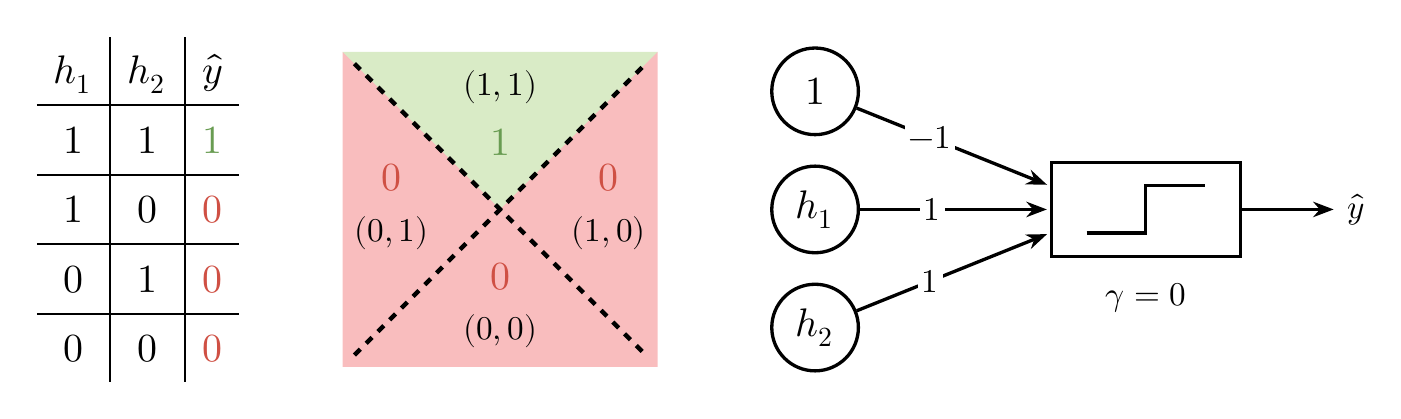
\begin{tikzpicture}
\node[font=\Large] at (0,1.5) {\setlength{\arrayrulewidth}{0.8pt}\renewcommand{\arraystretch}{1.35}%
\begin{tabular}{c|c|c}
$h_1$ & $h_2$ & $\hat y$ \\
\hline
$1$ & $1$ & {\color{green}$1$} \\
\hline
$1$ & $0$ & {\color{red}$0$} \\
\hline
$0$ & $1$ & {\color{red}$0$} \\
\hline
$0$ & $0$ & {\color{red}$0$} \\
\end{tabular}};

\begin{scope}[shift={(2.6,-0.5)}]
\fill[fillgreen, fill opacity=0.7] (0,4) -- (4,4) -- (2,2) -- cycle;
\fill[fillred, fill opacity=0.7] (0,4) -- (2,2) -- (4,4) -- (4,0) -- (0,0) -- cycle;
\draw[black, line width=1.6pt, dashed] (0.15,3.85) -- (3.85,0.15);
\draw[black, line width=1.6pt, dashed] (0.15,0.15) -- (3.85,3.85);
\node[font=\Large, text=green] at (2,2.85) {$1$};
\node[lbl] at (2,3.55) {$(1, 1)$};
\node[font=\Large, text=red] at (0.62,2.4) {$0$};
\node[lbl] at (0.62,1.7) {$(0, 1)$};
\node[font=\Large, text=red] at (3.38,2.4) {$0$};
\node[lbl] at (3.38,1.7) {$(1, 0)$};
\node[font=\Large, text=red] at (2,1.15) {$0$};
\node[lbl] at (2,0.45) {$(0, 0)$};
\end{scope}

\begin{scope}[shift={(8.6,0)}]
\node[neuron] (b)  at (0,3) {$1$};
\node[neuron] (h1) at (0,1.5) {$h_1$};
\node[neuron] (h2) at (0,0) {$h_2$};
\node[block, minimum width=24mm, minimum height=12mm] (f) at (4.2,1.5) {};
\draw[plain] ($(f.center)+(-0.75,-0.3)$) -- ($(f.center)+(0,-0.3)$) -- ($(f.center)+(0,0.3)$) -- ($(f.center)+(0.75,0.3)$);
\node[lbl, below=2mm of f] {$\gamma = 0$};
\draw[edge] (b)  -- ($(f.west)+(0,0.3)$)  node[wl, pos=0.38] {$-1$};
\draw[edge] (h1) -- (f.west)               node[wl, pos=0.38] {$1$};
\draw[edge] (h2) -- ($(f.west)+(0,-0.3)$) node[wl, pos=0.38] {$1$};
\draw[edge] (f.east) -- ++(1.2,0) node[lbl, right] {$\hat y$};
\end{scope}
\end{tikzpicture}
\end{document}
